\scanpage{30}\mspage{29}
% @ top, proposition heading
\uline{Proposition} Soient $F',F,G$ trois figures.
% @ top, three implications
\[
\begin{aligned}
 \text{a)}\quad F'\ll F&\Longrightarrow F'.G\ll F.G\\
 \text{b)}\quad F'\preceq F&\Longrightarrow F'.G\preceq F.G\\
 \text{c)}\quad F'\leq F&\Longrightarrow F'.G\leq F.G\quad{}^{*}
\end{aligned}
\]
% @ upper right, beside a
\margin{(trivial par \unsure{déf.|def.} de $\ll$ comme Inf)}
% @ upper right, beside b
\margin{(\unsure{résulte} de a), en regardant supports)}
% @ upper left, starred gloss
\margin{$*$ \uline{\unsure{explicitation|expliciter|explicitons}}}
% @ upper part, starred formula
\[
 F'.G=\{A\in F.G\mid A\subset |F'|\}
\]

% @ upper part, proof lines 1–2
Prouvons c. Il faut prouver que \deleted{$F'.G$} $F'.G\subset F.G$, et est fermé dans $F.G$.

% @ middle, proof lines 1–5
\deleted{\unsure{or}} Or $F'.G$ est formé des $A\cap B$ $(A\in F',B\in G)$ tels que $A^\circ\cap B^\circ\ne\varnothing$, et $F.G$ des $A\cap B$ $(A\in F,B\in \unsure{L|G})$ tels que $A^\circ\cap B^\circ\ne\varnothing$, et dans les deux cas le \unsure{sens} de $A^\circ$ (p.r. à $F$, \unsure{ds|dans} $F'$) est le $=$, donc $F'.G\subset F.G$. Prouvons que c'est fermé i.e.
% @ centre, first membership and annotations
Si \deleted{$(A\cap B\qquad A,A'\in F,$}
\[
 \underset{\substack{\rotatebox{-90}{$\in$}\\ F'}}{A}\cap
 \underset{\substack{\rotatebox{-90}{$\in$}\\ G}}{B}\in F'.G\qquad
 \text{i.e. } A^\circ\cap B^\circ\ne\varnothing
\]
% @ centre, second membership and annotations
\[
 \underset{\substack{\rotatebox{-90}{$\in$}\\ F}}{A'}\cap
 \underset{\substack{\rotatebox{-90}{$\in$}\\ G}}{B'}\in\underset{\text{\inserted{i.e. $A'^\circ\cap B'^\circ\ne\varnothing$}}}{F.G},\qquad
 \text{et } A'\cap B'\subset A\cap B\ \deleted{\unsure{\text{i.e.}}},\quad\text{alors}
\]
% @ middle lower, conclusion lines 1–4
$A'\cap B'\in F'.G$ i.e. $A'\in F'$. Or on sait que (d'après la théorie de $F.G$) que $A'\cap B'\subset A\cap B\Longrightarrow A'\subset A$, $B'\subset B$, d'où $A'\in F'$ puisque $F'$ fermé dans $F$.

% @ lower left, oblique explanation
% slanted
\margin{\uline{Expliciter}~: soit
\diagram{\begin{tikzcd}[ampersand replacement=\&,column sep=small,row sep=small]
 G\arrow[r,phantom,"\leq" description]\&F\arrow[d,phantom,"\rotatebox{90}{$\preceq$}" description]\\
 {}\&F'
\end{tikzcd}}, d'où $G'$ avec $G'\preceq G$, $G'\leq F'$. Alors on a $G'=\{A'\in F'\mid A'\subset |G|\}=\varphi^{-1}(G)$, où $\varphi:F'\to F\ldots$}
% @ lower right, two notes and their separating rules
% The stepped boundary is open on the right, as on the sheet.
\margin{\figure{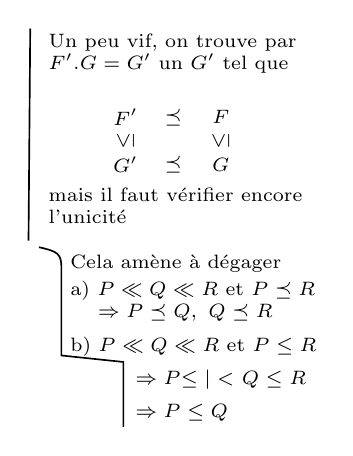
\begin{tikzpicture}[x=.55cm,y=.55cm,every node/.style={font=\scriptsize,inner sep=1pt}]
 \node[anchor=north west,text width=3.4cm] at (.35,0) {Un peu vif, on trouve par $F'.G=G'$ un $G'$ tel que};
 \node at (2.2,-2.0) {$F'$};
 \node at (3.3,-2.0) {$\preceq$};
 \node at (4.4,-2.0) {$F$};
 \node at (2.2,-2.55) {\rotatebox{90}{$\leq$}};
 \node at (4.4,-2.55) {\rotatebox{90}{$\leq$}};
 \node at (2.2,-3.1) {$G'$};
 \node at (3.3,-3.1) {$\preceq$};
 \node at (4.4,-3.1) {$G$};
 \node[anchor=north west,text width=3.4cm] at (.35,-3.55) {mais il faut vérifier encore l'\uline{unicité}};
 \draw[line width=.6pt] (0,.05) -- (-.04,-4.85);
 \node[anchor=north west,text width=3.2cm] at (.85,-5.1) {Cela amène à dégager};
 \node[anchor=north west,align=left] at (.85,-5.7) {a) $P\ll Q\ll R$ et $P\preceq R$\\\hspace*{.35cm}$\Rightarrow P\preceq Q,\ Q\preceq R$};
 \node[anchor=north west,align=left] at (.85,-7.0) {b) $P\ll Q\ll R$ et $P\leq R$};
 \node[anchor=north west] at (2.35,-7.75) {$\deleted{\Rightarrow P\unsure{\leq|<}}\ Q\leq R$};
 \node[anchor=north west] at (2.35,-8.55) {$\Rightarrow P\leq Q$};
 \draw[line width=.6pt] (.2,-5.0) .. controls (.65,-5.1) and (.72,-5.15) .. (.72,-5.5)
 -- (.72,-7.5) -- (2.15,-7.65) -- (2.15,-9.15);
\end{tikzpicture}}}
% @ lower part, corollary
\uline{Cor}. L'axiome C6 est valable.

% @ lower part, introduction to C7
Vérifions quand même C$7_0$
% @ lower part, order diagram and existence
\diagram{\begin{tikzcd}[ampersand replacement=\&,column sep=small,row sep=small]
 G\arrow[r,phantom,"\leq" description]\arrow[d,phantom,"\rotatebox{90}{$\preceq$}" description]\&F\& {\exists\ \text{subdivision }F'\text{ de }F\text{ qui}}\\
 G'\& {}\&{\text{induise }G'.}
\end{tikzcd}}
% @ bottom, construction
On prend $F'=G'\cup\deleted{\unsure{(F.G)}}(F\setminus G)$ (réunion disjointe)
% @ bottom, verification items
Il faut vérifier a) c'est une figure b) \unsure{qui|que} \deleted{\unsure{raffine}}\inserted{subdivise} $F$ et c) qui induit $G'$ sur $G$.
